\documentclass[12pt, eng, oneside, openany, final]{mgr}
% \documentclass[eng, printmode]{mgr}


% PREAMBULA


%% Language and font encodings
\usepackage[polish]{babel}
\usepackage[utf8x]{inputenc}
\usepackage[T1]{fontenc}

%% Sets page size and margins
\usepackage[a4paper,top=3cm,bottom=2cm,left=3cm,right=3cm,marginparwidth=1.75cm]{geometry}
%% \usepackage[a4paper, left=2.5cm, right=2.5cm, top=2.5cm, bottom=2.5cm, headsep=1.2cm]{geometry} -- Domski 

%% linki w spisie tresci, bibliografi
\usepackage[bookmarks=true,bookmarksnumbered=false,unicode=true,colorlinks=true,filecolor=black,linkcolor=black,urlcolor=black,citecolor=black]{hyperref}

\usepackage[colorinlistoftodos]{todonotes}

\usepackage{multirow} %tabele scalone
\usepackage{pdfpages} %wstawianie PDF'ów

%OPEROWANIE NA OBRAZACH
\usepackage{graphicx}       % pakiet graficzny, umożliwiający m.in.
% import grafik w formacie eps
%\usepackage{epstopdf}		% pozwala na importowanie grafik w formacie eps
% przy użyciu pdflatex
\usepackage[update,prepend]{epstopdf}
\usepackage{rotating}       % pakiet umożliwiający obracanie rysunków
\usepackage{subfigure}      % pakiet umożliwiający tworzenie podrysunków
\usepackage{epic}           % pakiet umożliwiający rysowanie w środowisku latex
\usepackage{psfrag}         % pakiet umożliwiający podmianę łańcuchów znaków 
% w plikach eps
%\usepackage{curves}         % pakiet do wykreslania krzywych

%pakiety dodające dużo dodatkowych poleceń matematycznych
\usepackage{amsfonts}       % pakiet z rozmaitymi czcionkami matematycznymi
% \usepackage{amssymb}        % pakiet z rozmaitymi symbolami matematycznymi
\usepackage{amsmath}        % pakiet z rozmaitymi środowiskami matematycznymi

\usepackage{fp}             % pakiet z funkcjami operujacymi 
% na liczbach zmiennoprzecinkowych
\usepackage{calc}           % pakiet umożliwiający operacje arytmetyczne
% na tzw. licznikach (liczbach całkowitych)
\usepackage{leftidx}		% indeksy górne i dolne po lewej stronie

%definicje matematyczne
\providecommand{\abs}[1]{\lvert#1\rvert}
\providecommand{\norm}[1]{\lVert#1\rVert}

%pakiety wspomagające i poprawiające składanie tabel
\usepackage{supertabular}
\usepackage{array}
\usepackage{tabularx}
\usepackage{hhline}
\usepackage{longtable}		% wsparcie dla dlugich tabel
\usepackage{multicol}		% podzial strony na wiele kolumn

%pakiet do BibTex
\usepackage{cite}

\usepackage{url} %pakiet pozawalający na dodawanie adresów url w bibliografi

%pakiet wypisujący na marginesie etykiety równań i rysunków zdefiniowanych przez \label{}, chcąc wygenerować finalną wersję dokumentu wystarczy usunąć poniższą linię
%\usepackage{showlabels}

\usepackage{float}			% lepsza obsluga mechanizmow obiektow plywajacych
% wymuszenie wstawienia np. tabeli, obrazka w danym miejscu przez [H]

\usepackage[]{siunitx} %jednostki np micro

\usepackage{listings}       % pakiet dedykowany zrodlom programow
\usepackage{color}


\definecolor{dkgreen}{rgb}{0,0.6,0}
\definecolor{gray}{rgb}{0.5,0.5,0.5}
\definecolor{mauve}{rgb}{0.58,0,0.82}

\lstset{ %
	language=Matlab,                % the language of the code
	basicstyle=\scriptsize,           % the size of the fonts that are used for the code
	numbers=left,                   % where to put the line-numbers
	numberstyle=\tiny\color{gray},  % the style that is used for the line-numbers
	stepnumber=1,                   % the step between two line-numbers. If it's 1, each line 
	% will be numbered
	numbersep=5pt,                  % how far the line-numbers are from the code
	backgroundcolor=\color{white},      % choose the background color. You must add \usepackage{color}
	showspaces=false,               % show spaces adding particular underscores
	showstringspaces=false,         % underline spaces within strings
	showtabs=false,                 % show tabs within strings adding particular underscores
	%frame=single,                   % adds a frame around the code
	rulecolor=\color{black},        % if not set, the frame-color may be changed on line-breaks within not-black text (e.g. comments (green here))
	tabsize=2,                      % sets default tabsize to 2 spaces
	captionpos=b,                   % sets the caption-position to bottom
	breaklines=true,                % sets automatic line breaking
	breakatwhitespace=false,        % sets if automatic breaks should only happen at whitespace
	%title=\lstname,                   % show the filename of files included with \lstinputlisting;
	% also try caption instead of title
	keywordstyle=\color{blue},          % keyword style
	commentstyle=\color{dkgreen},       % comment style
	stringstyle=\color{mauve},         % string literal style
	escapeinside={\%*}{*)},            % if you want to add LaTeX within your code
	morekeywords={*,...},              % if you want to add more keywords to the set
	deletekeywords={...}              % if you want to delete keywords from the given language
}

%polish signs in lst code
\lstset{literate=%
	{ą}{{\k{a}}}1
	{ć}{{\'c}}1
	{ę}{{\k{e}}}1
	{ł}{{\l}}1
	{ń}{{\'n}}1
	{ó}{{\'o}}1
	{ś}{{\'s}}1
	{ż}{{\.z}}1
	{ź}{{\'z}}1
	{Ą}{{\k{A}}}1
	{Ć}{{\'C}}1
	{Ę}{{\k{E}}}1
	{Ł}{{\L}}1
	{Ń}{{\'N}}1
	{Ó}{{\'O}}1
	{Ś}{{\'S}}1
	{Ż}{{\.Z}}1
	{Ź}{{\'Z}}1
}

\usepackage{verbatim}       % pakiet dedykowany rozmaitym wydrukom tekstowym
\usepackage{ifthen}         % pakiet umożliwiający tworzenie prostych programów
% (m.in. zawiera instrukcje powtórzeniowe 
% i warunkowe)
\usepackage{upquote}		%normal quotations marks ' and `

% deklaracje wymagane przez pakiet theorem automatycznie ladowany w przypadku
% klasy dokumentu article
%
\newtheorem{Dn}{Definicja}[section]     % deklaracja srodowiska definicja
\newtheorem{La}[Dn]{Lemat}                % deklaracja srodowiska lemat
\newtheorem{Tm}[Dn]{Twierdzenie}          % deklaracja srodowiska twierdzenie
\newtheorem{Rk}[Dn]{Spostrze{\.z}enie}  % deklaracja srodowiska spostrzezenie
\newtheorem{Am}[Dn]{Algorytm}           % deklaracja srodowiska algorytm
\newtheorem{As}[Dn]{Za{\l}o{\.z}enie}   % deklaracja srodowiska zalozenie
\newtheorem{Pn}[Dn]{Propozycja}           % deklaracja srodowiska propozycja
\newtheorem{Py}[Dn]{W{\l}asno{\'s}{\'c}}  % deklaracja srodowiska wlasnosc
\newtheorem{Cy}[Dn]{Wniosek}              % deklaracja srodowiska wniosek
\newtheorem{Ee}[Dn]{Przyk{\l}ad}        % deklaracja srodowiska przyklad
\newtheorem{Ex}{{\'C}wiczenie}          % deklaracja srodowiska cwiczenie

\newtheorem{theorem}{Twierdzenie}[section] %nowe otoczenie do składania twierdzeń
%definicje własnych poleceń
\newcommand{\R}{I\!\!R} %symbol liczb rzeczywistych, działa tylko w trybie matematycznym

%helps to specify width of a column in table
%\begin{tabular}{|C{1cm}|c|c|c|c|c|c|c|c|c|c|}
%first column will have widht of 1cm
\newcolumntype{L}[1]{>{\raggedright\let\newline\\\arraybackslash\hspace{0pt}}m{#1}}
\newcolumntype{C}[1]{>{\centering\let\newline\\\arraybackslash\hspace{0pt}}m{#1}}
\newcolumntype{R}[1]{>{\raggedleft\let\newline\\\arraybackslash\hspace{0pt}}m{#1}}

\sloppy			%zawija bardzo długie linie

%\pagenumbering{gobble}% Remove page numbers (and reset to 1)

% \include{bibliografia}


% re-definiowane polecenie w celu przechowywania nazwiska autora, jego brak powoduje ostrzezenie (Warning) podczas przetwarzania.
\author{Jakub Adam Taczała} 

% re-definiowane polecenie w celu przechowywania polskiego tytułu pracy magisterskiej, jego brak powoduje ostrzezenie (Warning) podczas przetwarzania.
\title{Omijanie przeszkód przez robota mobilnego poruszającego się wzdłuż linii} 


% polecenie zdefiniowane w celu przechowywania angielskiego tytułu pracy magisterskiej, jego brak powoduje ostrzezenie (Warning) podczas przetwarzania.
\engtitle{Obstacle avoidance by the linefollower mobile robot} 


% polecenie zdefiniowane w celu przechowywania danych osobowych prowadzacego prace, jego brak powoduje ostrzezenie (Warning) podczas przetwarzania.
\supervisor{Dr inż. Janusz Jakubiak} 

% polecenie zdefiniowane w celu przechowywania danych osobowych opiekuna pracy. W przypadku gdy jest to ta sama osoba co \supervisor, nie nalezy uzywac tego polecenia. Jego brak usunie ze strony tytułowej zbedna informacje.
%\guardian{tytuł, Imie Nazwisko, jednostka} 


% polecenie zdefiniowane w celu przechowywania nazwy kierunku studiów, jego brak powoduje ostrzezenie (Warning) podczas przetwarzania.
\field{Automatyka i Robotyka (AIR)} 


% polecenie zdefiniowane w celu przechowywania nazwy specjalnosci studiów, jego brak powoduje ostrzezenie (Warning) podczas przetwarzania.
\specialisation{Robotyka (ARR)} 

% re-definiowane polecenie w celu przechowywania roku. Standardowo u dołu strony tytułowej wstawiany jest biezacy rok, uzycie tego polecenia pozwala wstawic dowolny rok.
\date{2018} 



\begin{document}
\maketitle
% polecenie w miejscu swojego wystapienia łamie biezaca strone i na nastepnej (w przypadku openright na nastepnej prawej) wstawia po prawej u dołu tresc dedykacji z argumentu tekst. Argument szer musi miec wartosc sztywnej długosci i definiuje szerokosc pola tekstowego z trescia dedykacji.
\dedication{6cm}{Pracę dedykuję Ojcu, za motywację, wytrwałość i pokazanie jak dążyć do celu mimo przeciwności. \texttt{Dziękuję}}

\tableofcontents
\listoffigures
\listoftables

\newpage
\chapter{Wprowadzenie}
Dążenie człowieka do odnalezienie drogi do celu jest obecne od zarania dziejów. O podążaniu po wyznaczonej ścieżce wspomina już bowiem mitologia grecka w micie pt. ,,Dzieje Tezeusza'', gdzie bohater by wyjść po nitce z labiryntu musiał zmierzyć się z przeszkodą -- Minotaurem\cite{mitologia}. Wraz z ewolucją powstawały coraz to nowsze możliwości podążania do celu wraz z omijaniem przeszkód. Obecny Postęp techniki pozwala by realizacje tego celu powierzyć robotom autonomicznym. Owe choć w uproszczony sposób są w stanie samodzielnie podejmować podstawowe decyzje, jednakże strategiczne decyzje wciąż musi podejmować człowieka. Sposobów na rozwiązanie tego problemu wciąż przybywa, co sprzyja rozwojowi technologii.
\section{Cel i zakres pracy}
Celem pracy jest zastosowanie czujników ultradźwiękowych oraz czujników odbiciowych do budowy robota autonomicznego poruszającego się po czarnej linii, potrafiącego ominąć przeszkodę postawioną na owej trasie. Z tego powodu konieczne jest rozpoznanie możliwości oraz opracowanie algorytmu poruszania się robota po wyznaczonej ścieżce, wraz z omijaniem przeszkód i powrotem na wyznaczoną ścieżkę, zakładając iż otoczenie nie zwraca nam odpowiedzi o aktualnym położeniu robota. Projekt jest połączeniem szczególnych cech robotów typu Line Follower oraz Micromouse.
Funkcje robota:
\begin{itemize}
    \item określenie toru jazdy względem czarnej linii na białym podłożu na podstawie czujnika odbiciowego;
    \item określenie odległości od przeszkody za pomocą czujników ultradźwiękowych;
    \item poruszanie się wzdłuż przeszkody określając odległość od niej za pomocą czujników ultradźwiękowych;
    %\item określenie przebytego dystansu na podstawie zliczania ilości kroków silników krokowych;
    \item ponowne odnalezienie linii zadającej tor jazdy za pomocą czujników zbudowanych na fotodiodach podczas poruszania się wzdłuż przeszkody.
\end{itemize}

\section{Możliwe zastosowania}
Robot w większej formie może być wykorzystywany w wielu projektach.
\begin{itemize}
    \item Jako autonomiczny wózek systemowy do transportu towaru w magazynach o dużej przestrzeni. Z podobnego systemu korzystają niektóre sortownie paczek w firmach kurierskich.
    \item Zastosowanie w postaci podstawy platformy do robota mobilnego z manipulatorem. Robot taki mógłby poruszać się w magazynach niskiego składu. A zastosowanie efektora pozwoliło by na przenoszenie pojedynczych sztuk towarów.
    \item Wykorzystanie do budowy modułu podstawy autonomicznego wózka widłowego w magazynach wysokiego składu. Zastosowanie robota autonomicznego w takich warunkach pozwala uniknąć narażania pracowników na wypadek związany z upadkiem towaru z półek. Pozwoli także na precyzyjne, powtarzalne ustawianie palet na półkach wysokiego składu w taki sposób by nie miał możliwości osunięcia się z konstrukcji. Natomiast zastosowanie czujników ultradźwiękowych pozwoli na wyminiecie innego robota, który zatrzymał się np. z powodu awarii, bądź ominięcie innej przeszkody, która nie powinna znajdować się na trasie.
\end{itemize}
\newpage 
\chapter{Opis budowy robota}
\section{Wstęp}
Rozdział przedstawia zadania postawione przed robotem, które są do zrealizowania w ramach pracy inżynierskiej. Zawarte jest w nim także porównanie podobnych konstrukcji, których fragmenty zostały przeanalizowane i wybrane do budowy konstrukcji. Zawiera też opis użytych modułów wraz z argumentacją wyboru.
\section{Zadania do realizacji przez robota}
\begin{itemize}
    \item \textbf{Przetworzenie informacji o położeniu względem wyznaczonej ścieżki}
    Na podstawie pomiaru uzyskanego z czujników odbiciowych znajdujących się nad zakreśloną trasą wprowadzana jest korekta trajektorii.
    \item \textbf{Obserwacja otoczenia}
    Na podstawie pomiaru uzyskanego z czujników ultradźwiękowych znajdujących się na czole robota określenie odległości od przeszkody i próba ominięcia jej.
    \item \textbf{Analiza informacji o położeniu wału silnika}
    Zapisywanie kroków przebytych przez każde z kół po zjechaniu z linii.
    \item \textbf{Wyznaczenie położenia robota}
    Wyznaczenie odległości przebytej od punktu porzucenia trasy w skutek napotkania przeszkody.
    \item \textbf{Próba powrotu na ścieżkę }
    Poprzez zachowanie bliskiej odległości od przeszkody próba powrotu na ścieżkę.
    \item \textbf{Podjęcie decyzji o ewentualnym niepowodzeniu zadania}
    W momencie osiągnięcia położenia początkowego, bądź oddalenia się zbytnio od linii podjęcie decyzji o zatrzymaniu platformy.
\end{itemize}

\section{Podobne konstrukcje}
Robot jest połączeniem dwóch klasycznych konstrukcji, robota podążającego po linii oraz robota omijającego przeszkody.

Roboty podążające po linii często wykorzystują czujniki własnej konstrukcji zbudowane z użyciem transoptorów. Takie podejście pozwala dostosować kształt wiązki czujników do kształtu maszyny, jednakże wymaga własnego projektu modułu. Często takie rozwiązania odczytują bezpośrednio napięcie z fotodiody, przez co konieczne jest wykorzystanie przetwornika ADC.\cite{line_czujnik} Problem ten można rozwiązać prze dodanie kondensatorów, a następnie pomiar czasu ich rozładowania na portach I/O procesora, tak jak to zostało wykonane w projekcie. 

Dobrym rozwiązaniem do kontroli otoczenia jest zastosowanie czujników odległości na czole pojazdu. \cite{line_sharp} Jednakże zastosowanie czujników ultradźwiękowych pozwala uzyskać większy kąt pomiaru, a także mniejszą wrażliwość na chropowate powierzchnie ze względu na szerokość wiązki fali czołowej. Robot spełniający podobne zadania, jednakże bez funkcji omijania przeszkody wyposażony w czujnik ultradźwiękowy może pełnić funkcje robota przemysłowego jako wózek AGV, który to jest wykorzystywany do transportu towarów w magazynie. \cite{AGV}

Dość innowacyjnym sposobem jest zastosowanie silników krokowych do napędu robota mobilnego. Jednakże takie rozwiązanie pozwala na dokładne sterowanie w otwartej pętli sterowania, tym samym na bieżąco jest śledzona pozycja robota.\cite{kurosz} Takie rozwiązanie wiąże się jednocześnie z ograniczeniem prędkości robota w porównaniu do użycia innych silników prądu stałego.\cite{Tadeo} W przedstawionej pracy jednakże nie zależy na uzyskaniu prędkości przejazdu, a w precyzji sterowania, by możliwie jak najdokładniej określić położenie robota względem linii.

\section{Opis zastosowanych modułów}
Podrozdział zawiera opis zastosowanych czujników wraz z uzasadnieniem wyboru w ramach projektu. Wybory te są wynikiem analizy konstrukcji mających spełniać zbliżone zadania. Tym samym sprawdzana jest stosowność doboru elementów.
\subsection{Opis konstrukcji typu Line Follower -- czujniki linii}
Celem konstrukcji jest podążanie po wyznaczonej trasie. Podczas zawodów robotycznych jest wykorzystywana czarna linia na kontrastowym białym podłożu, co pozwala robotowi na jednoznaczne określenie trasy poprzez użycie czujników odbiciowych składających się z par: dioda  IR razem z fototranzystorem. Dodatkowo poprzez włącznie w obwód kondensatorów pozwala na cyfrowy odczyt wartości poprzez pomiar czasu rozładowania danego kondensatora. W projekcie został użyty gotowych moduł składający się z ośmiu par takich czujników.
\begin{figure}[H]
\centering
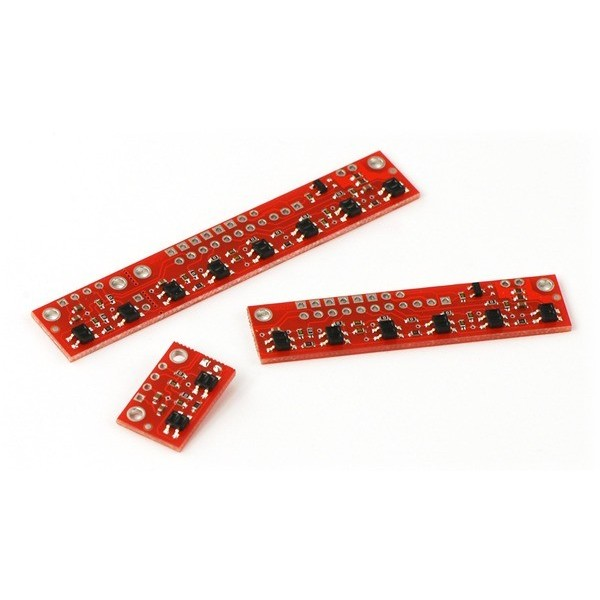
\includegraphics[width=0.5\textwidth]{inzynierku/img/listwa.jpg}
\caption{\label{fig:czujnik_odbiciowy}Listwa z czujnikami odbiciowymi QTR-8RC - cyfrowa.}
\end{figure}

\subsection{Opis konstrukcji typu Micromouse -- czujniki odległości}
Jest to robot, którego głównym zadaniem jest rozpoznawanie odległości do ściany. W przypadku tego projektu odległości do przeszkody. W celu realizacji owego zadania można wykorzystać jeden z wielu typów czujników odległości. Porównanie typów czujników zostało zawarte w Tablicy~\ref{tab:odleglosc}. W projekcie został użyty czujnik ultradźwiękowy.

\begin{table}[H]
\centering
\begin{tabular}{c|c|c}
\textbf{Rodzaj czujnika}        & \textbf{Zalety}           & \textbf{Wady}                     \\ \hline
\multirow{4}{*}{Ultradźwiękowe} & Kąt: \textless 15°        & Martwa strefa 2 cm                \\
                                & Dokładność: 0,3 cm + 1 \% & Czuły na chropowatość powierzchni \\
                                & Napięcie zasilania: 5 V   &                                   \\
                                & Pobór prądu 3 mA          &                                   \\ \hline
\multirow{2}{*}{Typu SHARP}     & Prostota implementacji    & Zasięg od 10 cm                   \\
                                &                           & Pobór prądu 33 mA                 \\ \hline
\multirow{2}{*}{Laserowe}       & Brak martwej strefy       & Czujnik cyfrowy                   \\
                                &                           & Punktowe działanie               
\end{tabular}
\caption{\label{tab:odleglosc}Zalety i wady danych typów czujników w zastosowaniu budowy robota podążającego po linii z funkcja omijania przeszkód. \cite{czujniki, sharp, laser}} 
\end{table}
\begin{figure}[H]
\centering
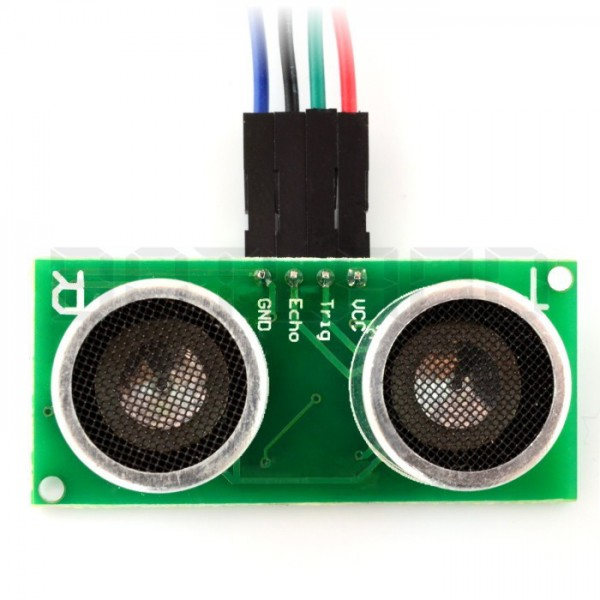
\includegraphics[width=0.5\textwidth]{inzynierku/img/czujnik.jpg}
\caption{\label{fig:czujnik_ultradzwiekowy}Ultradźwiękowy czujnik odległości US-015 2-400cm.}
\end{figure}

\subsection{Dobór silników}
Biorąc pod uwagę brak odpowiedzi z otoczenia na temat położenia robota względem przeszkody w otoczeniu należy pobierać dane o jego przybliżonym położeniu bezpośrednio z silników. Ze względu na rozmiar pracy odrzuca się silniki prądu zmiennego. Jednym z możliwych rozwiązań jest zastosowanie modelarskich silników prądu stałego, jednakże to rozwiązanie wymaga zastosowanie enkoderów do określenia przybliżonego położenia robota. Z tego powodu sensownym jest użycie silników krokowych, za pomocą których przybliżone położenie robota otrzymujemy już zadając ruch. Duża waga, ponad $220g$ każdego z silników pozwala zwiększyć siłę grawitacji $F_g=mg$, co pozytywnie wpływa na docisk kół do podłoża przez co zmniejszony jest efekt poślizgu. Celem platformy nie jest pokonanie trasy w jak najkrótszym czasie, prze co waga nie wpływa negatywnie na właściwości robota. W projekcie użyte są dwa silniki krokowe, posiadają one następujące właściwości:
\begin{itemize}
    \item rozdzielczość $1,8^\circ$;
    \item napięcie znamionowe wynoszące $12,0 V$;
    \item pobór prądu na cewkę $0,4 A$;
    \item moment trzymający $0,25 Nm$.
\end{itemize}
\begin{figure}[H]
\centering
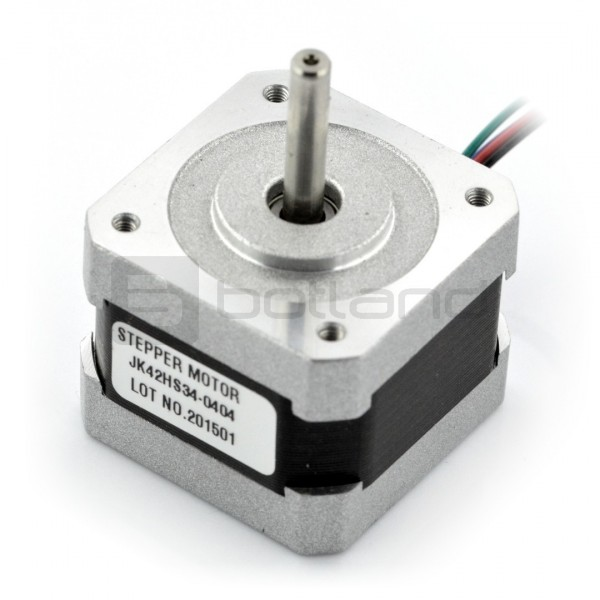
\includegraphics[width=0.5\textwidth]{inzynierku/img/silnik.jpg}
\caption{\label{fig:silnik_krokowy}Silnik krokowy JK42HS34-0404 200 kroków.}
\end{figure}

\subsection{Dobór sterowników silników}
Ze względu na problematyczność sterowania silnikami oraz prądy płynące przez silniki w projekcie użyto gotowych modłów do sterowania silnikiem. Dobierając takich moduł należy zwrócić uwagę na napięcie znamionowe silników, oraz zapotrzebowanie prądowe. Sterownik silnika należy dobrać z zapasem. Zastosowanie owego modułu pozwala na sterowanie silnikiem jedynie za pomocą dwóch wyjść z płytki uruchomieniowej. Na sterownik podawane są sygnały:
\begin{itemize}
    \item kroku;
    \item kierunku obrotu.
\end{itemize}
\begin{figure}[H]
\centering
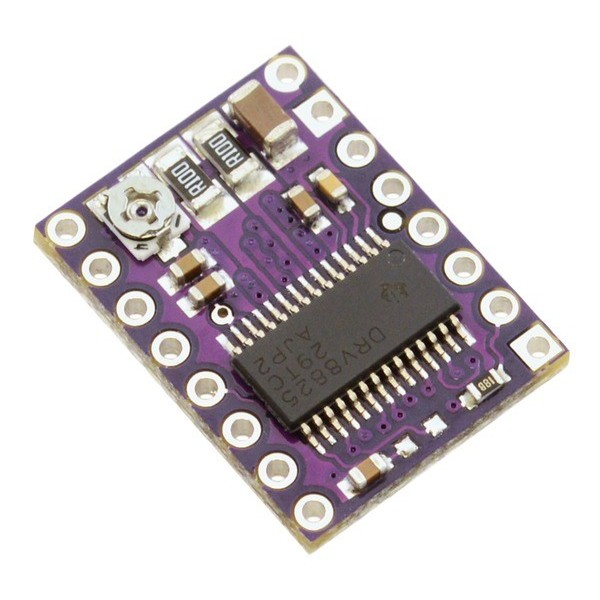
\includegraphics[width=0.5\textwidth]{inzynierku/img/sterownik.jpg}
\caption{\label{fig:sterownik_silnika}Pololu DRV8825 - sterownik silnika krokowego 45V/2,2A.}
\end{figure}

\subsection{Podział zasilania}
Z konieczności wykorzystania różnych napięć w projekcie wykorzystywany jest moduł o napięciach wyjściowych $3,3V$ oraz $5V$ z wydajnością prądową do $800mA$ na każdym z napięć. Napięcia $5V$ potrzebne są do zasilania czujników, oraz mikroprocesora.
\begin{figure}[H]
\centering
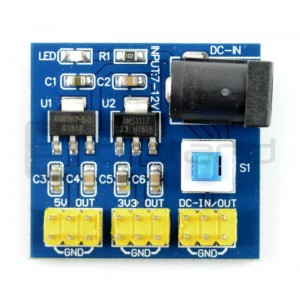
\includegraphics[width=0.5\textwidth]{inzynierku/img/zasilajacy.jpg}
\caption{\label{fig:modul_zasilajacy}Moduł zasilający 3,3V / 5V.}
\end{figure}

\subsection{Stabilizacja napięcia z baterii}
Do ustabilizowania napięcia ze źródła zasilania używana jest przetwornica. Przetwornica w porównaniu do stabilizatorów liniowych wydziela mniejsza ilość ciepła, a także pozwala na pracę z napięciem wejściowym mniejszym od napięcia wyjściowego. Użycie przetwornicy wymaka jednakże filtrację napięcia za pomocą kondensatorów. Zastosowanie tego elementu pozwala także na przetwarzanie wyższych natężeń prądu niż stabilizator. W projekcie przewidziane jest zasilanie bateryjne, jednakże silniki potrzebują napięcia 12V, które ma na celu dostarczyć chronić przed spadkami napięcia spowodowanym rozładowaniem źródła zasilania.
\begin{figure}[H]
\centering
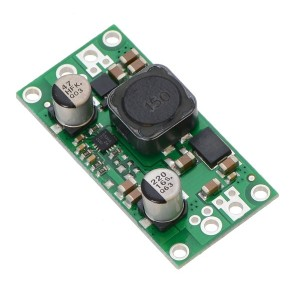
\includegraphics[width=0.5\textwidth]{inzynierku/img/przetwornica.jpg}
\caption{\label{fig:przetwornica_up_down}Pololu S18V20F12 - przetwornica step-up/down - 12V 2A.}
\end{figure}

\subsection{Płytka rozruchowa}
Płytką użytą w projekcie jest klon Arduino MEGA. Wybór tej płytki jest bezpośrednio powiązany z faktem, iż producenci często udostępniają biblioteki do obsługi czujników dla tego właśnie środowiska. Ze względu na liniowy charakter algorytmu, oraz niskie obciążenie procesora nie ma potrzeby wykorzystywania rozwiązań konkurencji, zawierających obsługę przerwań czy DMA. Użycie innego środowiska wiąże się z przepisaniem bibliotek. Płytka w użytej wersji zawiera:
\begin{itemize}
    \item 54 cyfrowych wejść/wyjść cyfrowych;
    \item w tym 15 można wykorzystać jako wyjścia PWM;
    \item 16 wejść analogowych;
    \item zegarowym o częstotliwości 16 MHz;
    \item 256 kB pamięci programu Flash;
    \item 8 kB pamięci operacyjnej SRAM;
    \item UART;
    \item I2C;
    \item SPI.
\end{itemize}
\begin{figure}[H]
\centering
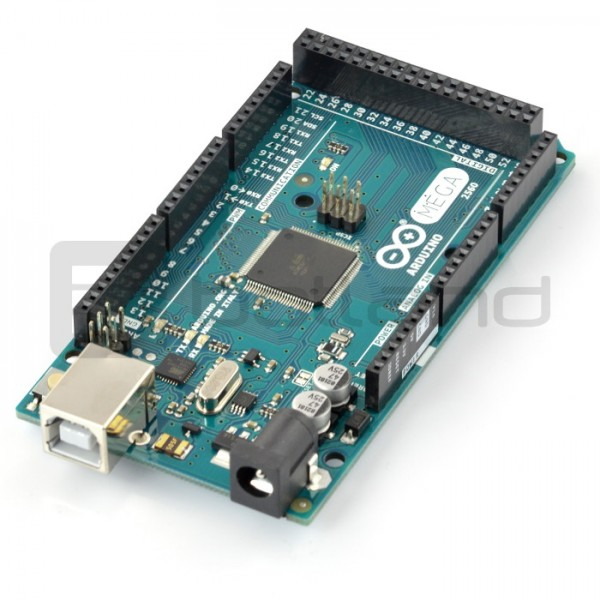
\includegraphics[width=0.5\textwidth]{inzynierku/img/arduino.jpg}
\caption{\label{fig:Arduino_MEGA}Płytka rozruchowa Arduino MEGA.}
\end{figure}

\section{Opis i schemat połączeń}
Podział zasilania zrobiony jest na płytce stykowej, natomiast sygnały podpięte są bezpośredni do płytki rozruchowej.
%\begin{figure}[H]
%\centering
%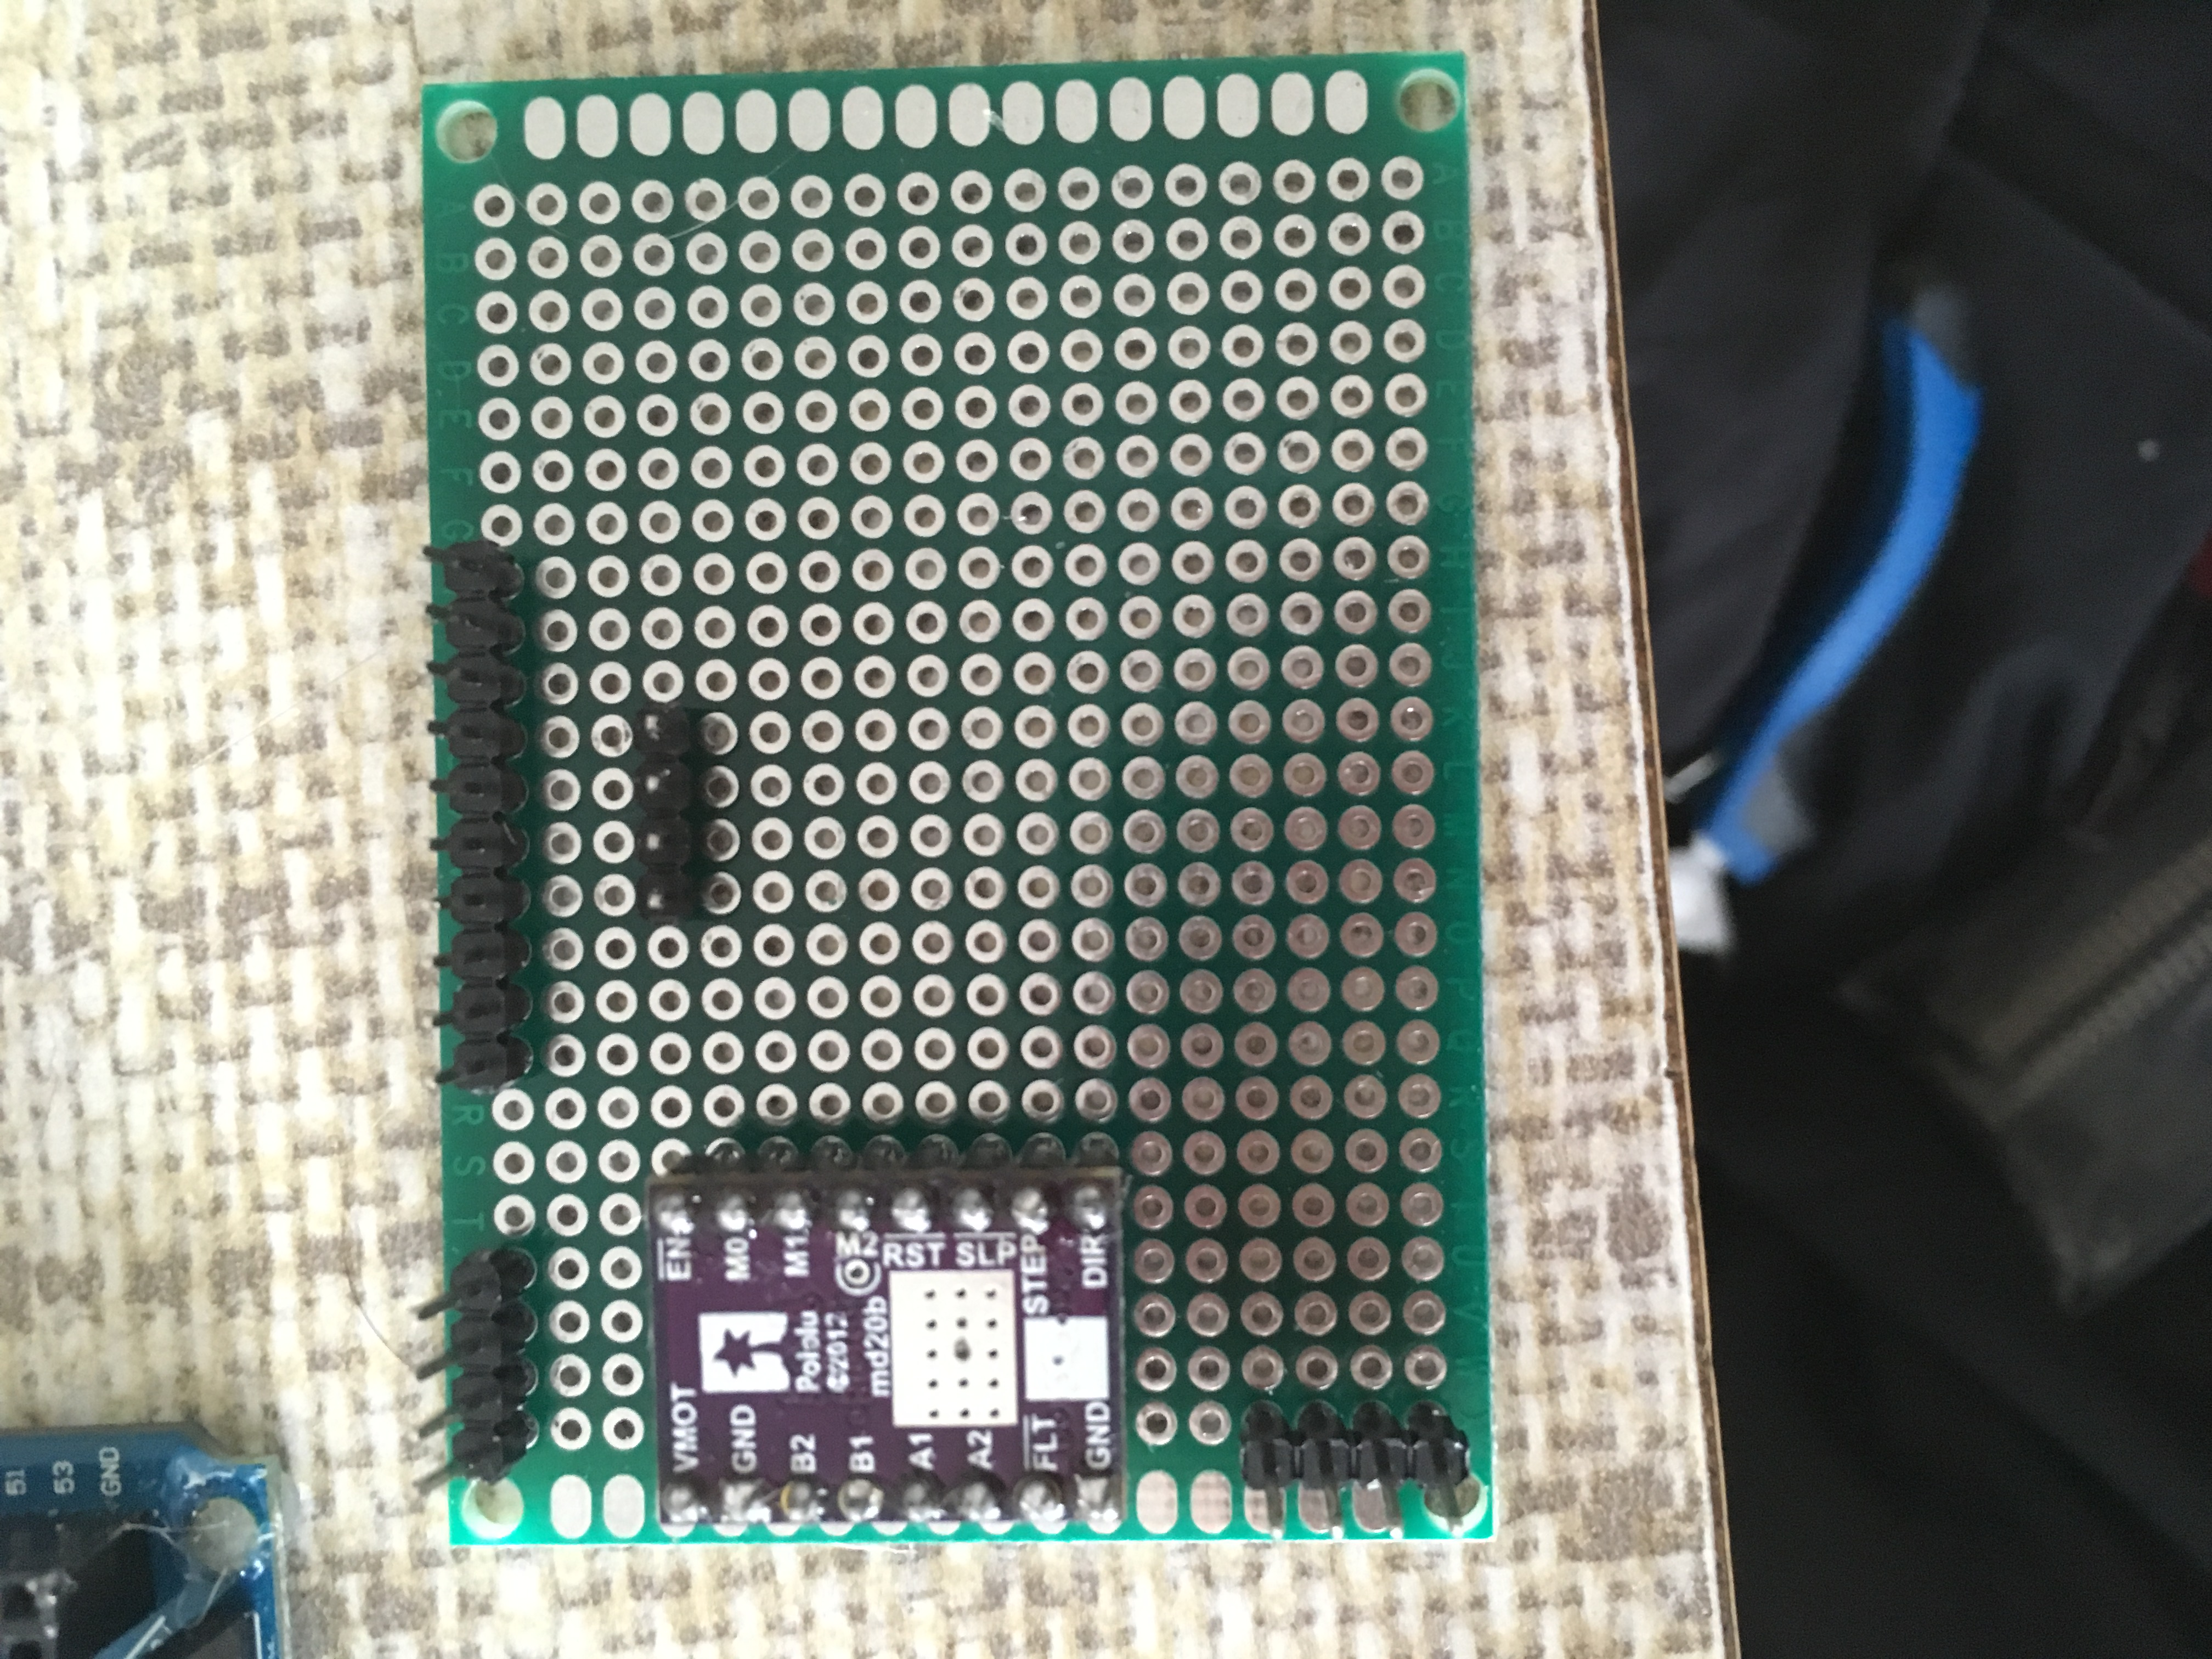
\includegraphics[width=0.5\textwidth]{inzynierku/img/plytka.jpg}
%\caption{\label{fig:plytka}Moduł podziału sygnałów i zasilania.}
%\end{figure}

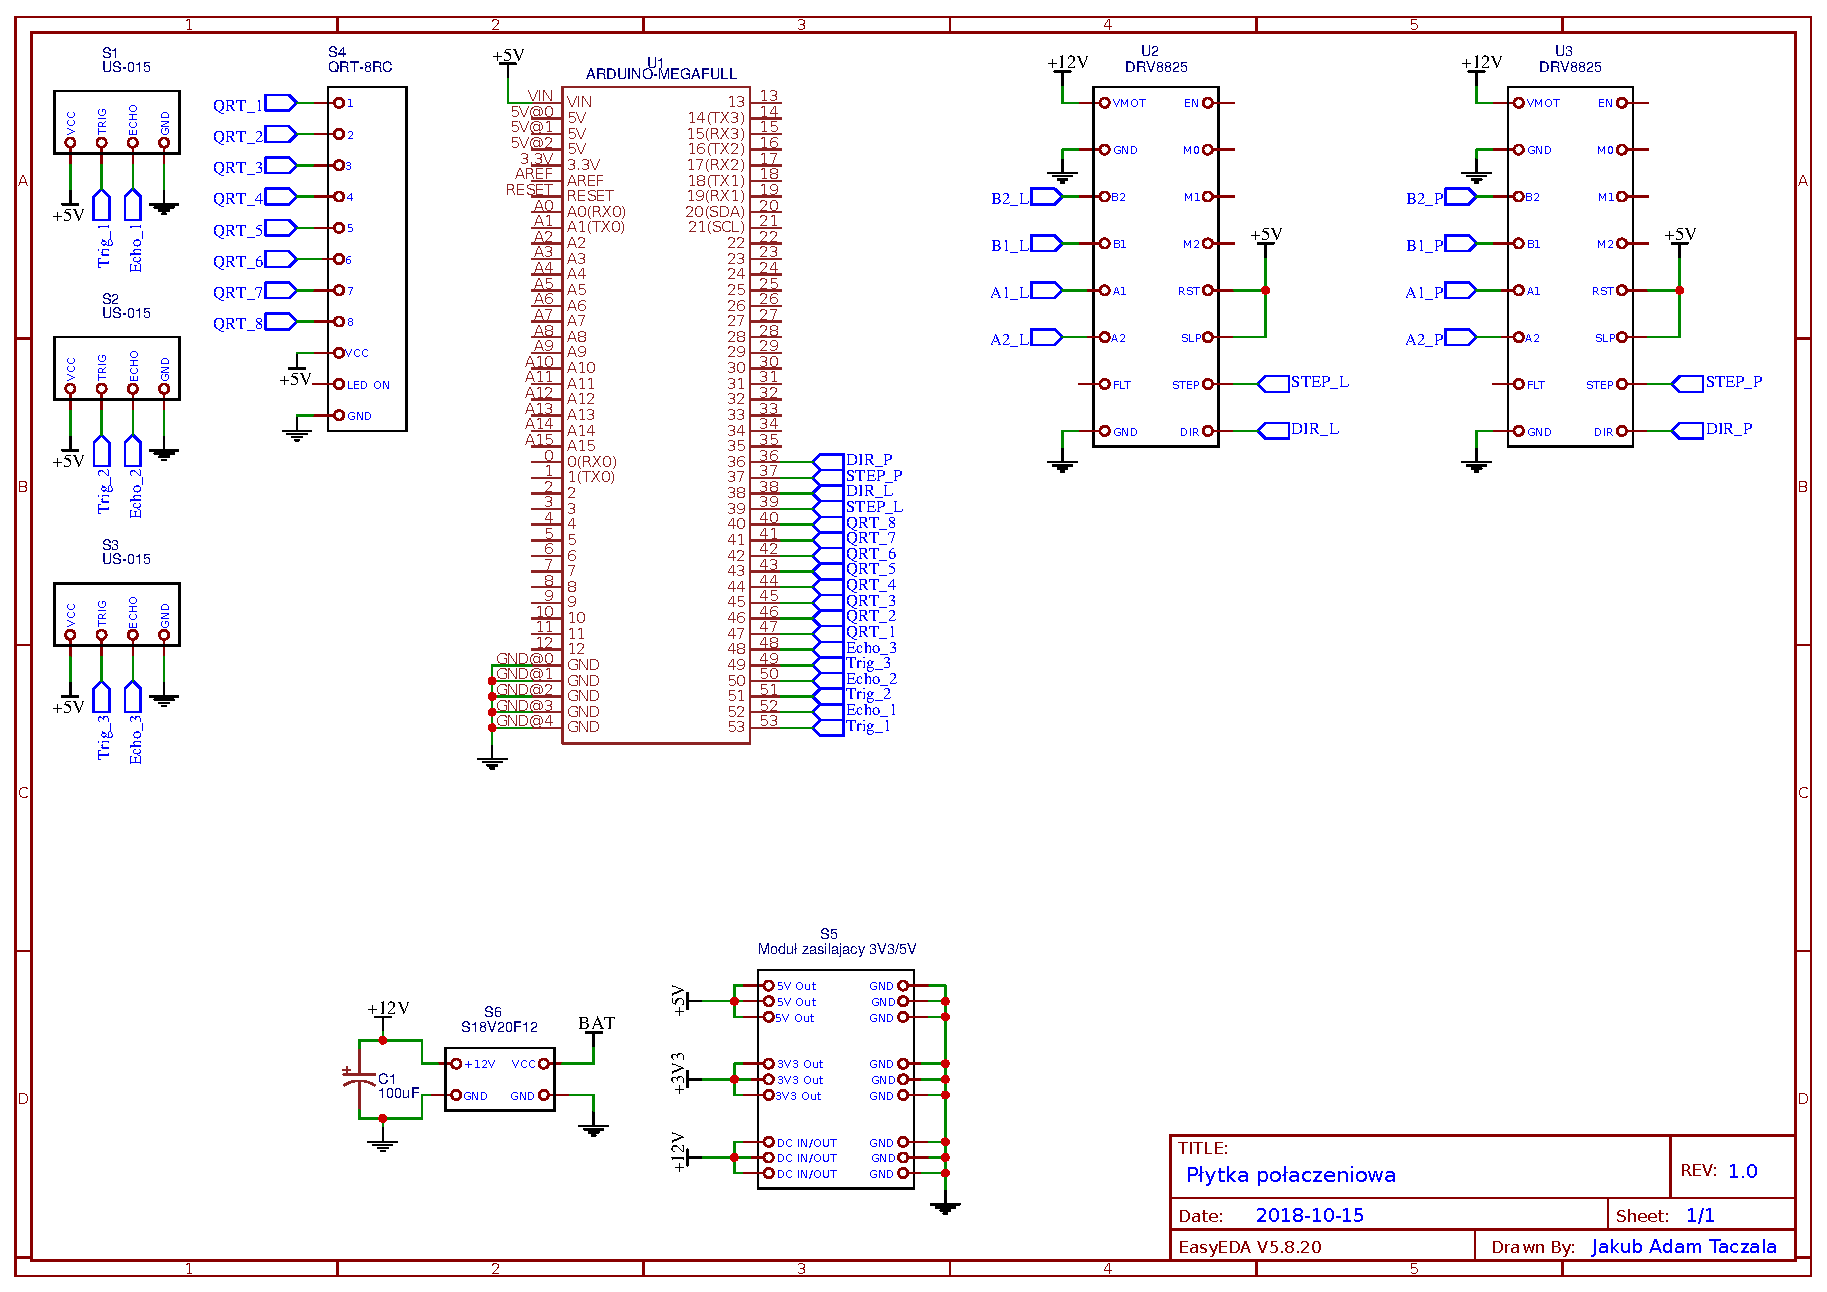
\includepdf{schematic.pdf}

\chapter{Problem podążania po wyznaczonej ścieżce}
\begin{figure}[H]
\centering
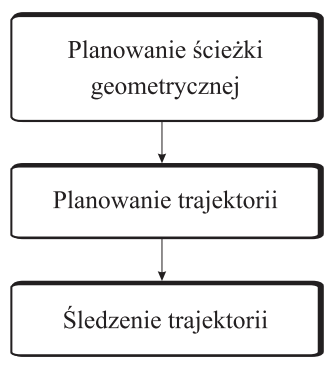
\includegraphics[width=0.5\textwidth]{inzynierku/img/planowanie.png}
\caption{\label{fig:planowanie}Planowanie ruchu \cite{planowanie_ruchu}.}
\end{figure}
Zadanie planowania ścieżki można podzielić na trzy etapy:
\begin{enumerate}
    \item Planowanie ścieżki geometrycznej -- wybór sposobu poruszania się robota, tj. czy platforma ma poruszać się do przodu czy też ma przyjąć rotację w jedna ze stron.
    \item Planowanie trajektorii -- określenie o ile kroków ma się poruszać w danym kierunku.
    \item Śledzenie trajektorii -- Na podstawie danych odbieranych przez czujniki określenie czy zadana trajektoria nie odbiega od zamierzonej ścieżki.
\end{enumerate}
Roboty mobilne o małej prędkości $V_{max}$ takie jak robot wykonany w projekcie, ze względu na niskie oddziaływanie sił bezwładności często są traktowane jako układy holonomiczne. \cite{planowanie_ruchu} W przypadku osiągania dużych prędkości przez robota należał oby uwzględnić poślizg kół, jednakże przez nagromadzenie wielu zmiennych wpływających wówczas na trajektorię, należy skorzystać z odpowiedzi otoczenia o położeniu układu.

W przypadku robota w układzie (2, 0) można skorzystać z metody halsowania znanej ze sposobu poruszania się łodzi żaglowych pod wiatr. Metoda ta pozwala na to by zawsze choć jeden czujnik znajdował się nad linią, jednocześnie upraszcza to sterowanie robotem jedynie do jazdy prawym bądź lewym kołem w przód.

W razie potrzeby porzucenia linii, najbezpieczniejszą metodą jest utrzymywanie robota w stałej odległości od przeszkody próbując ja w ten sposób ominąć przeszkodę i powrócić na linię. Jednakże ze względu na nieznajomość otoczenia należy uwzględnić sytuacje, w której to przeszkoda znajduje się np. w futrynie i po przebyciu określonej odległości zaprzestać kontynuacji zadania.

\section{Przyjęte ograniczenia robota oraz środowiska}
W ramach przedstawionego problemu przyjęto następujące uproszczenia:
\begin{enumerate}
    \item Robot jest jedynym obiektem przemieszczającym się w przestrzeni.
    \item Przestrzeń po której porusza się robot jest płaska.
    \item Przestrzeń po której porusza się robot jest gładka.
    \item Między kołami robota, a podłożem panuje idealna przyczepność.
    \item Podłoże jest białe, a ślad po którym porusza się robot wyznacza czarna linia.
    \item Pomieszczenie jest oświetlone przynajmniej na poziomie 300 luxów.
\end{enumerate}

\section{Ograniczenia robota wynikające z konstrukcji robota}
\begin{enumerate}
    \item Koła porusza się z prędkością nie większą niż $100RPM$.
    \item Obiekt do ominięcia znajduje się na wysokości czujników ultradźwiękowych.
    \item Korytarz po którym porusza robot nie może być węższy niż 38cm.
    \item Przed wypuszczeniem robota na trasę należy przeprowadzić kalibrację czujników.
    \item Napięcie zasilania wynosi $3V-30V$.
\end{enumerate}
% http://sequoia.ict.pwr.wroc.pl/~mucha/Robotyka/tchon_manipulatory_i_roboty_mobilne.pdf str. 268
\newpage 
\chapter{Implementacja algorytmów}
Środowiskiem implementacji algorytmów jest ARDUINO 1.8.7 w wersji na system operacyjny Mac OS Mojave w wersji 10.14.
\section{Opis implementacji wybranych funkcji startowych}
W programie została użyta biblioteka dostarczona przez firmę Pololu do czujnika QRT-8RC QTRSensors.h w wersji 3.1.0.\cite{QRT} Do poprawnego działania czujnika zalecana jest kalibracja, która odbywa się zaraz po uruchomieniu robota.
Do odczytu wartości wykorzystywana jest funkcja:
\begin{lstlisting}[language=C]
    void qtrrc.read(sensorValues);
\end{lstlisting}
następnie za pomocą własnej funkcji:
\begin{lstlisting}[language=C]
    int QRT_ktory_widzi();
\end{lstlisting}
wyznaczany jest czujnik, który znajduje się nad linią.
\\
\\
W celu uruchomienia czujnika ultradźwiękowego US-015  wykonano sekwencje:
\begin{itemize}
    \item pin $TRIG$ ustawiony na stan niski;
    \item opóźnienie 2\si{\micro}s;
    \item pin $TRIG$ ustawiony na stan wysoki;
    \item opóźnienie 10\si{\micro}s;
    \item pin $TRIG$ ustawiony na stan niski.
\end{itemize}
\begin{figure}[H]
\centering
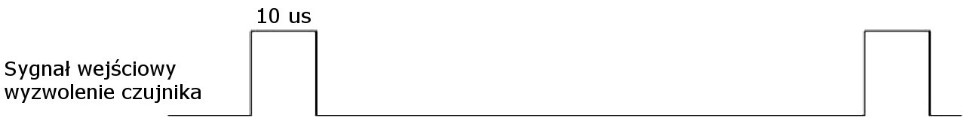
\includegraphics[width=0.9\textwidth]{inzynierku/img/sekwencja}
\caption{\label{fig:sekwencja}Sekwencja uruchomienia czujnika ultradźwiękowego.}
\end{figure}
Do sterowania silnikami zostały napisane trzy bliźniacze funkcje.
\begin{itemize}
    \item do sterowania lewym kołem
    \begin{lstlisting}[language=C]
    void stepperRotate_L(float rotation, float rpm);
    \end{lstlisting}
    \item do sterowania prawym kołem
    \begin{lstlisting}[language=C]
    void stepperRotate_P(float rotation, float rpm);
    \end{lstlisting}
    \item do sterowania dwoma kołami na raz -- jazda do przodu bądź do tyłu
    \begin{lstlisting}[language=C]
    void stepperRotate_S(float rotation, float rpm);
    \end{lstlisting}
\end{itemize}
Wszystkie wyżej wymienione funkcje przyjmują argumenty $rotation$ oraz $rpm$, które określają następująco ilość obrotów oraz prędkość obrotów.
W celu jazdy do przodu na pin $DIR$ należy podać sygnał wysoki, natomiast przy jeździe do tyłu stan niski.

\section{Opis algorytmu}
Działanie rozpoczyna się od kalibracji czujników wykrywania linii. Następnie przeprowadzana jest próba wykrycia przeszkody, jeśli owa zakończy się negatywnie, to robot próbuje podążać po linii. Podążanie po linii trwa dopóty robot nie natrafi na przeszkodę, gdzie ocenia którą stroną może ją ominąć, bądź zgłasza brak możliwości minięcia. Po ominięciu przeszkody kontynuuje jazdę po linii wyszukując następną przeszkodę powracając do fazy podążania po linii. Dokładny algorytm przedstawiony jest na rysunku \ref{fig:schemat_blokowy}.
\section{Graf algorytmu}
\begin{figure}[H]
\centering
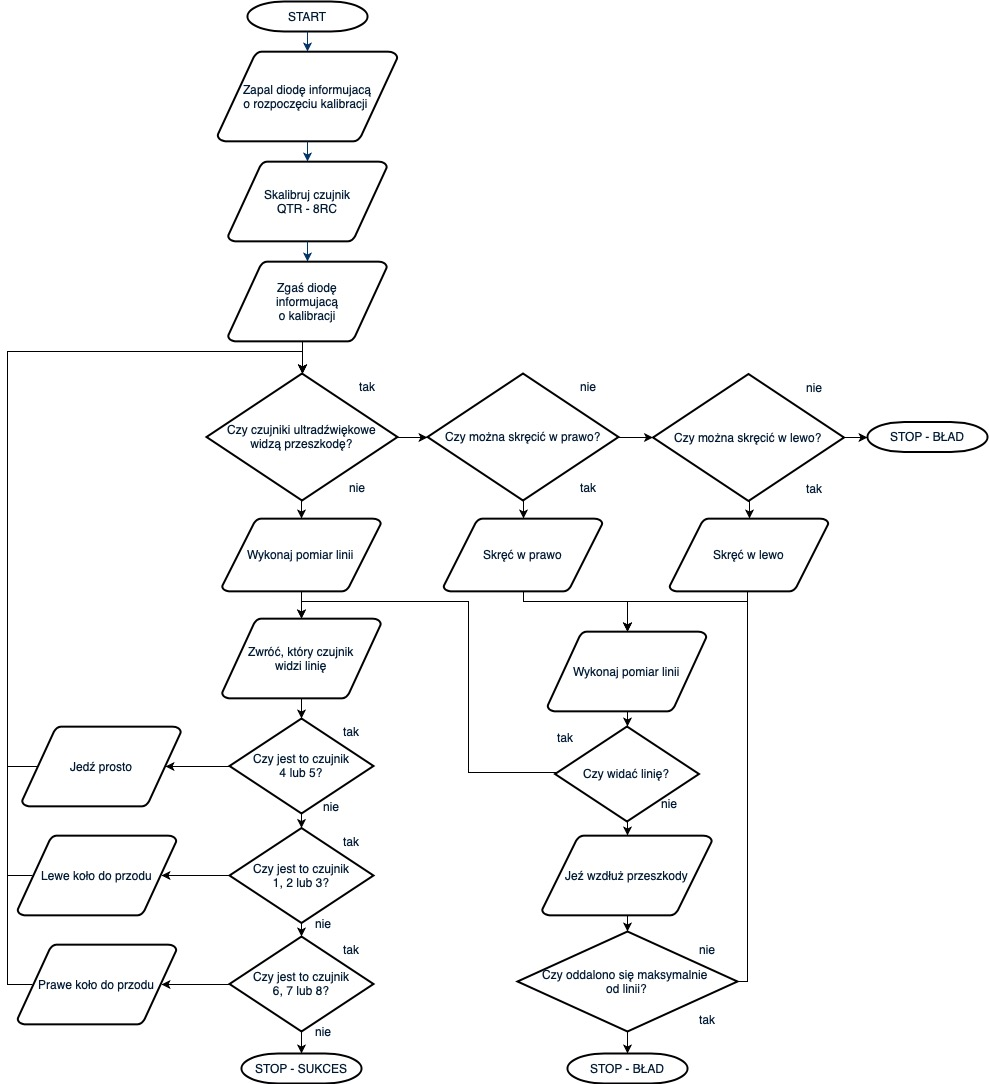
\includegraphics[width=\textwidth]{inzynierku/img/diagram}
\caption{\label{fig:schemat_blokowy}Schemat blokowy sterowania.}
\end{figure}
\newpage 
\chapter{Testy}
\section{Test podążania po linii}
\subsection{Cel testu}
Test ma na celu sprawdzenie poprawności implementacji czujników odbiciowych wraz z wykazaniem poprawności integracji silników z odczytami.
\subsection{Opis testu}
\subsection{Rezultaty testu}

\section{Test wykrywania przeszkody}
Test ma na celu sprawdzenie poprawności implementacji czujników ultradźwiękowych wraz z wykazaniem poprawności integracji silników z odczytami.
\subsection{Cel testu}
\subsection{Opis testu}
\subsection{Rezultaty testu}

\section{Test podążania wzdłuż przeszkody}
Test ma na celu sprawdzenie zachowania podczas utrzymywania stałej odległości od przeszkody, tym samym sprawdzenie poprawności omijania przeszkody.
\subsection{Cel testu}
\subsection{Opis testu}
\subsection{Rezultaty testu}

\section{Test powrotu na linię}
Test ma na celu sprawdzenie zachowania po ominięciu przeszkody i wykazania, czy robot jest w stanie powrócić na tor jazdy.
\subsection{Cel testu}
\subsection{Opis testu}
\subsection{Rezultaty testu}
\newpage 
\chapter{Podsumowanie}
\section{Zadania wykonane w ramach pracy}
W ramach pracy dyplomowej został stworzony robot w układzie (2, 0). Przeanalizowano konstrukcje, korzystające z podobnych metod określenia położenia w otoczeniu. Na tej podstawie dobrano czujnik wykrywania linii, czujniki ultradźwiękowe oraz sposób napędzania platformy z zastosowaniem silników krokowych. Po zapoznaniu się z dobranymi czujnikami zdecydowano o płytce rozruchowej kierując się wymaganiami specyfikacji określonymi przez czujniki.

Analizując sposoby poruszania się wspomnianych robotów zaprojektowano algorytm dla tworzonego projektu. Uwzględniono ograniczenia, jakie wynikają z zastosowanych czujników, Następnie zaimplementowano czujniki i algorytm sterowania. 

Gotową konstrukcje przetestowano sprawdzają poprawność implementacji, poddając ją próbom w rzeczywistym otoczeniu. Podczas testów została określona poprawność toru jazdy przy pomocy czujnika odbiciowego. Przeprowadzono również pomiary odległości od przeszkody czujnikami ultradźwiękowymi. Wykorzystując owe pomiary określono sposób poruszania się przy przeszkodzie. Natomiast zliczanie kroków pozwoliło na określenie przybliżonego dystansu pokonanego od startu robota, wraz z określeniem odległości poza wyznaczoną trasą. Korzystając z zastosowanych modułów wykonano próby odnalezienia linii wyznaczającej dalszy tor jazdy, podczas poruszania się wzdłuż omijanego przedmiotu.

\section{Uzyskane rezultaty}
UZUPEŁNIĆ!!!!!!!!!!!!!!!!

\section{Możliwe rozszerzenia}
Do celów wykrywania przeszkody oraz określenia położenia względem niej, a także śledzenia linii można zastosować kamerę, co pozwoli na ograniczenie ilości czujników. Takie rozwiązanie wymaga większej mocy obliczeniowej do celu przetwarzania uzyskanego obrazu.

Kolejnym rozszerzeniem może być użycie większej ilości zastosowanych czujników uzyskując tym samym podgląd na otoczenie w każdym kierunku.

%\input{inzynierku/przyklady.tex}

\bibliographystyle{plabbrv}

\addcontentsline{toc}{chapter}{Bibliografia} %utworzenie w spisie treści pozycji Bibliografia
\bibliography{bibliografia} % wstawia bibliografię korzystając z pliku bibliografia.bib - dotyczy BibTeXa, jeżeli nie korzystamy z BibTeXa należy użyć otoczenia thebibliography

\end{document}